\documentclass[
	% -- opções da classe memoir --
	12pt,				% tamanho da fonte
	openright,			% capítulos começam em pág ímpar (insere página vazia caso preciso)
	oneside,			% para impressão em recto e verso. Oposto a oneside
	a4paper,			% tamanho do papel. 
	% -- opções da classe abntex2 --
	chapter=TITLE,		% títulos de capítulos convertidos em letras maiúsculas
	%section=TITLE,		% títulos de seções convertidos em letras maiúsculas
	%subsection=TITLE,	% títulos de subseções convertidos em letras maiúsculas
	%subsubsection=TITLE,% títulos de subsubseções convertidos em letras maiúsculas
	% -- opções do pacote babel --
	english,			% idioma adicional para hifenização
	brazil,				% o último idioma é o principal do documento
	]{abntex2}

% ---
% Pacotes fundamentais 
% ---
\usepackage{unijui}

\usepackage[utf8]{inputenc}		% Codificacao do documento (conversão automática dos acentos)
\usepackage{indentfirst}		% Indenta o primeiro parágrafo de cada seção.
\usepackage{color}				% Controle das cores
\usepackage{graphicx}			% Inclusão de gráficos
\usepackage{microtype} 			% para melhorias de justificação
% ---

% ---
% Pacotes de citações
% ---
\usepackage[brazilian]{}

\usepackage{placeins}
\usepackage{multirow}
\usepackage[table]{xcolor}
\usepackage[pt-BR]{datetime2}


\DTMlangsetup{showdayofmonth=false}

% ---
% Informações de dados para capa, folha de rosto e folha de aprovação
% ---
\titulo{Trabalho exemplo que obedece às normas de formatação ABNT da UNIJUI}
\autor{Nome do Autor}
\local{Santa Rosa, Brasil}
\data{\today}
\instituicao{%
   Universidade Regional do Noroeste do Estado do Rio Grande do Sul - UNIJUI}
\orientador{Prof. Dr. Orientador}
\tipotrabalho{Trabalho de Conclusão de Curso}
% O preambulo deve conter o tipo do trabalho, o objetivo, 
% o nome da instituição e a área de concentração 
\preambulo{Trabalho de Conclusão de Curso apresentado ao curso de Bacharelado em Ciência da Computação da Universidade Regional do Noroeste do Estado do Rio Grande do Sul, como requisito parcial à obtenção do título de Bacharel em Ciência da Computação.}


% ---
% Configurações de aparência do PDF final


% informações do PDF
\makeatletter
\hypersetup{
     	%pagebackref=true,
		pdftitle={\@title}, 
		pdfauthor={\@author},
    	pdfsubject={\imprimirpreambulo},
	    pdfcreator={LaTeX with abnTeX2},
		pdfkeywords={tcc}{computação}{ciência}, 
		colorlinks=true,       		% false: boxed links; true: colored links
    	linkcolor=black,          	% color of internal links
    	citecolor=black,        		% color of links to bibliography
    	filecolor=black,      		% color of file links
		urlcolor=black,
		bookmarksdepth=4
}
\makeatother
% --- 

% --- 
% Espaçamentos entre linhas e parágrafos 
% --- 

% O tamanho do parágrafo é dado por:
\setlength{\parindent}{1.3cm}

% Controle do espaçamento entre um parágrafo e outro:
\setlength{\parskip}{0.2cm}

% ---
% compila o indice
% ---
\makeindex
% ---

% ----
% Início do documento
% ----
\begin{document}

% Seleciona o idioma do documento (conforme pacotes do babel)
%\selectlanguage{english}
\selectlanguage{brazil}

% Retira espaço extra obsoleto entre as frases.
\frenchspacing 

% ---
% Capa
% ---

\imprimircapa
% ---

% ---
% Folha de rosto
% ---

\imprimirfolhaderosto*

% ---

% ---
% Inserir a ficha bibliografica
% ---

% Isto é um exemplo de Ficha Catalográfica, ou ``Dados internacionais de
% catalogação-na-publicação''. Você pode utilizar este modelo como referência. 
% Porém, provavelmente a biblioteca da sua universidade lhe fornecerá um PDF
% com a ficha catalográfica definitiva após a defesa do trabalho. Quando estiver
% com o documento, salve-o como PDF no diretório do seu projeto e substitua todo
% o conteúdo de implementação deste arquivo pelo comando abaixo:
%
% \begin{fichacatalografica}
%     \includepdf{fig_ficha_catalografica.pdf}
% \end{fichacatalografica}

% ---
% Inserir folha de aprovação
% ---

% Modelo de folha de aprovação utilizado na UNIJUI, elemento obrigatório da NBR
% 14724/2011 (seção 4.2.1.3). Você pode utilizar este modelo até a aprovação
% do trabalho. Após isso, substitua todo o conteúdo deste arquivo por uma
% imagem da página assinada pela banca com o comando abaixo:
%
% \includepdf{folhadeaprovacao_final.pdf}
%


\newcommand{\imprimirfolhaaprovacao}{%
	\begin{folhadeaprovacao}		
	\begin{center}
		\ABNTEXchapterfont\mdseries\large\MakeUppercase\imprimirinstituicao
		
		\vspace*{5mm}
		
		A Comissão Examinadora, abaixo assinada, aprova o \imprimirtipotrabalho:
		
		\vspace*{5mm}
		
		\ABNTEXchapterfont\large\bfseries\MakeUppercase\imprimirtitulo\mdseries
		
		\vspace*{5mm}
		
		Elaborado por
		
		\vspace*{5mm}
		
		\ABNTEXchapterfont\mdseries\large\MakeUppercase\imprimirautor
		
		\vspace*{5mm}
		
		Como requisito parcial para obtenção do título de Bacharel em Ciência da Computação
		
		\vspace*{\fill}
		
		Comissão Examinadora
		
		\assinatura{\textbf{\imprimirorientador} \\ Orientador} 
		\assinatura{\textbf{Professor} \\ Convidado 1}
		\assinatura{\textbf{Professor} \\ Convidado 2}
		%\assinatura{\textbf{Professor} \\ Convidado 3}
	
		\vspace*{\fill}
		{\large\imprimirlocal}
		
		\par
		
		%A data de aprovação e as assinaturas dos membros componentes da banca examinadora devem ser colocadas após a aprovação do trabalho.		
		{\large 17 de Junho de 2017}
	\end{center}	
	\end{folhadeaprovacao}
}

\imprimirfolhaaprovacao

% ---

% ---
% Dedicatória
% ---
\begin{dedicatoria}
	\vspace*{\fill}
	\centering
	\noindent
	\textit{ Dedicatória, linha 1,\\
		linha 2.} \vspace*{\fill}
\end{dedicatoria}
% ---

% ---
% Agradecimentos
% ---
\begin{agradecimentos}
	Inserir os agradecimentos.	
\end{agradecimentos}
% ---

% ---
% Epígrafe
% ---
\begin{epigrafe}
	\vspace*{\fill}
	\begin{flushright}
		\textit{Texto de Epígrafe}
	\end{flushright}
\end{epigrafe}
% ---

% ---
% RESUMOS
% ---

% resumo em português
\setlength{\absparsep}{18pt} % ajusta o espaçamento dos parágrafos do resumo
\begin{resumo}

Resumo em português.

	\textbf{Palavras-chave}: Palavras chave. \textit{Relay}.
\end{resumo}

% resumo em inglês
\begin{resumo}[Abstract]
	\begin{otherlanguage*}{english}

Resumo em inglês.
		
		\vspace{\onelineskip}
		
		\noindent 
		\textbf{Keywords}: Arothmetic and Logic Unit. Processors. Computer Architecture.
	\end{otherlanguage*}
\end{resumo}


% ---
% inserir lista de ilustrações
% ---
\pdfbookmark[0]{\listfigurename}{lof}
\listoffigures*
\cleardoublepage

% ---
% inserir lista de tabelas
% ---
\pdfbookmark[0]{\listtablename}{lot}
\listoftables*
\cleardoublepage

\begin{siglas}
	\item[UCP] Unidade Central de Processamento (CPU - \textit{Central Processing Unit})
	\item[ENIAC] \textit{Electronic Numerical Integrator and Computer} - Computador Integrador Numérico Eletrônico
\end{siglas}

\begin{simbolos}
  \item[$ \mu $] Prefixo Micro
  \item[$ \wedge $] Operação Lógica E
  \item[$ \lor $] Operação Lógica OU
  \item[$ \oplus $] Operação Lógica OU exclusivo  
  \item[$ \lnot $] Operação Lógica de negação
\end{simbolos}

% ---
% inserir o sumario
% ---
\pdfbookmark[0]{\contentsname}{toc}
\tableofcontents*
\cleardoublepage
% ---


\textual

\chapter{Introdução}

Lorem ipsum dolor sit amet, consectetur adipiscing elit. Phasellus gravida lectus quis nisi maximus convallis. Sed congue feugiat nunc, blandit fringilla neque vehicula sit amet. Aliquam elementum nisl neque, id sollicitudin dui ornare eget. Integer et diam elementum eros ullamcorper porta quis lacinia justo. Vestibulum accumsan lectus in efficitur lacinia. Donec at dictum urna. Integer blandit lectus eu commodo consequat.

\chapter{Desenvolvimento}

Exemplo de citação \cite{einstein}.

Praesent scelerisque elit a interdum aliquam. Nullam varius ex eget elementum fermentum. Donec scelerisque velit arcu, nec pellentesque purus condimentum efficitur. Donec viverra libero felis, at bibendum ipsum pretium consequat. Sed sed tempus ipsum. Cras non lorem ornare, aliquet sapien id, maximus mi. Quisque sollicitudin urna venenatis laoreet rutrum. Duis viverra tellus sit amet eros imperdiet, eget aliquet urna venenatis. Nam a nunc vitae tortor fermentum convallis. Integer a aliquam arcu, in sodales nulla. Nulla nec ligula nec ligula pellentesque egestas vel eu lectus. Morbi consectetur eu mauris ac egestas. Nunc faucibus quis quam eget rhoncus. Nulla vitae dignissim erat, in aliquam justo. Aliquam facilisis odio nec dapibus vulputate. Fusce accumsan molestie augue at egestas.

\section{Seção Secundária}

Exemplo de citação \cite{turing}, referenciando o anexo \ref{turing_article}.

Exemplo de figura \ref{logo_unijui}:

\begin{figure}[h!]
	\centering
	\caption{\label{logo_unijui}Logo}
	
\includegraphics[scale=0.8]{imagens/logo-unijui-horizontal.png}
	\legend{Fonte: Unijui.}
\end{figure}
\FloatBarrier	

\subsection{Seção terciária}

Duis rhoncus, ligula bibendum ullamcorper pretium, neque ligula iaculis mauris, eget suscipit libero nunc sed mi. Aenean volutpat eu dolor hendrerit rhoncus. Vivamus in fringilla elit. Proin tincidunt molestie lacinia. Vivamus nunc felis, rutrum in neque id, congue ultricies ex. Ut eget lectus pharetra, lobortis purus sodales, gravida massa. Proin et interdum ipsum. Nunc non nibh feugiat, accumsan nisl vitae, iaculis leo. Nulla sodales porta egestas. Praesent commodo scelerisque risus eget porta. Suspendisse ut augue sed sapien auctor dictum. Morbi sodales euismod risus, id tincidunt lectus malesuada quis. Etiam volutpat neque id velit hendrerit, non tincidunt eros fringilla. Nam erat sem, imperdiet nec facilisis nec, vulputate at leo. Donec lorem urna, iaculis at mollis non, varius eu eros.

Exemplo de citação \cite{neumann}. Um exemplo de tabela pode ser visto na tabela \ref{tabela_peso}.

\begin{table}[htb]
	\IBGEtab{%
		\caption{Relação peso x altura}%
		\label{tabela_peso}
	}{%
		\begin{tabular}{ccc}
			\toprule
			\textbf{Peso X} & \textbf{Estatura Y} & \textbf{Idade Z}  \\
			\midrule
			35 & 128 & 13 \\
			39 & 125 & 14 \\
			41 & 123 & 15 \\
			33 & 120 & 12 \\
			\bottomrule
		\end{tabular}%
	}{%
		\fonte{O autor.}%
	}
\end{table}
\FloatBarrier

% ---
% Finaliza a parte no bookmark do PDF
% para que se inicie o bookmark na raiz
% e adiciona espaço de parte no Sumário
% ---
\phantompart

% ---
% Conclusão
% ---
\chapter{Conclusão}
% ---

Curabitur et lacus a risus eleifend rutrum. Sed lacinia consequat ex eu molestie. Ut tempus id neque ac faucibus. Duis tincidunt euismod justo et scelerisque. Vivamus malesuada felis lorem, et cursus nibh sodales eget. Aliquam erat volutpat. In pretium in eros in auctor. Nam lectus augue, consectetur vitae dui et, lacinia porttitor leo. Vivamus nec nibh nec nunc eleifend viverra vitae a arcu. Etiam venenatis euismod diam vel interdum. Sed bibendum ante laoreet felis laoreet, in aliquet massa sagittis. Etiam nunc orci, sagittis at pulvinar eget, tincidunt a arcu. Ut id ipsum sed velit vulputate viverra. Maecenas sed semper elit, in tincidunt nibh. Vestibulum finibus erat viverra tortor dictum vulputate. Aenean auctor, libero sed euismod feugiat, dui erat dictum eros, in cursus urna sapien nec neque.

\postextual

% ----------------------------------------------------------
% Referências bibliográficas
% ----------------------------------------------------------
\bibliography{bibliografia}


% ---
% Inicia os anexos
% ---

\begin{anexosenv}
	
	\partanexos
	
	\chapter{Turing Article}
	\label{turing_article}
	\begin{figure}[h!]
		\centering
		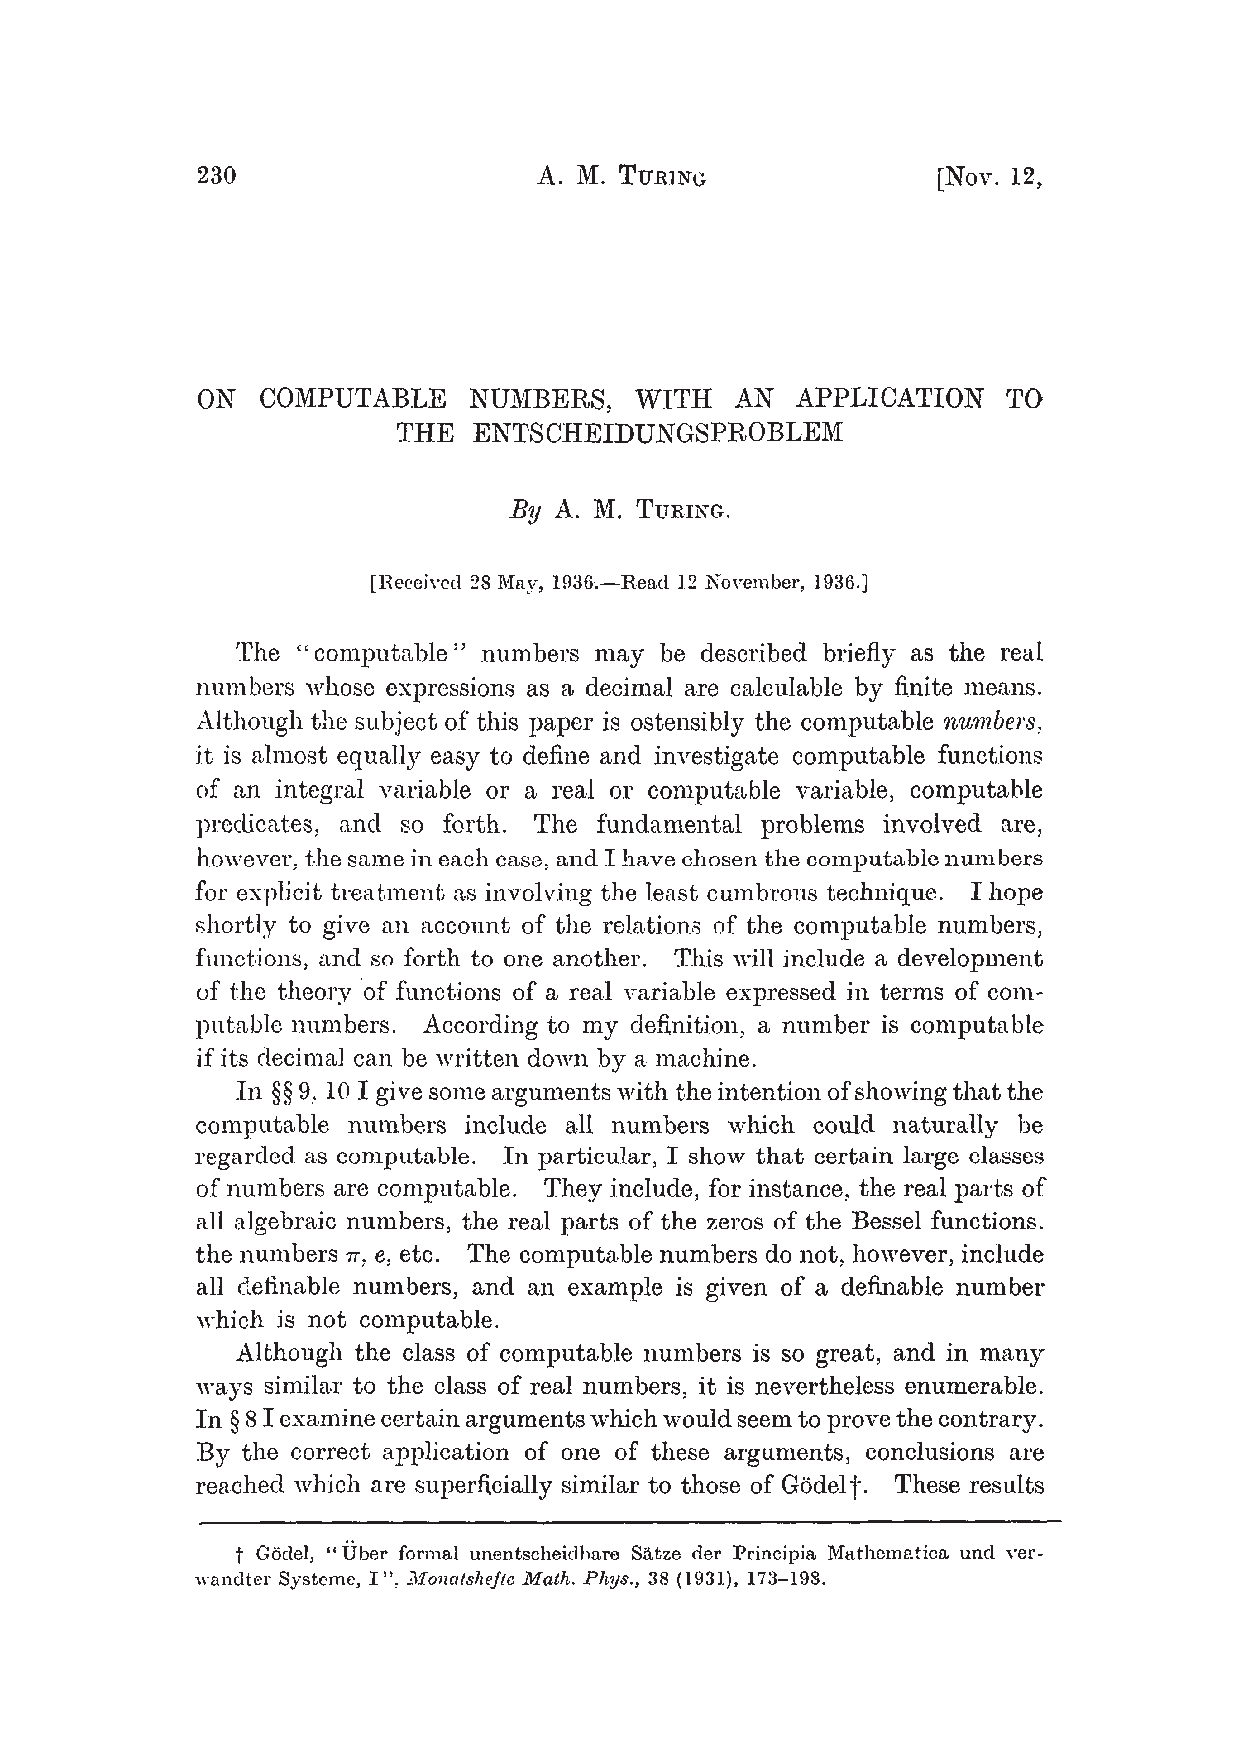
\includegraphics[page=1,trim={2.5cm 0 2cm 2cm},clip,scale=0.8]{anexos/turing.pdf}
	\end{figure}
	\FloatBarrier
	
\end{anexosenv}


\end{document}
